\begin{frame}
    \frametitle{D-Bus}
    Potrzeba zaimplementowania ustandaryzowanego,
    bezpiecznego IPC dla
    środowisk graficznych.

    2002 - początek projektu

    2006 - stabilna wersja
\end{frame}

\begin{frame}
    \frametitle{Działanie}
    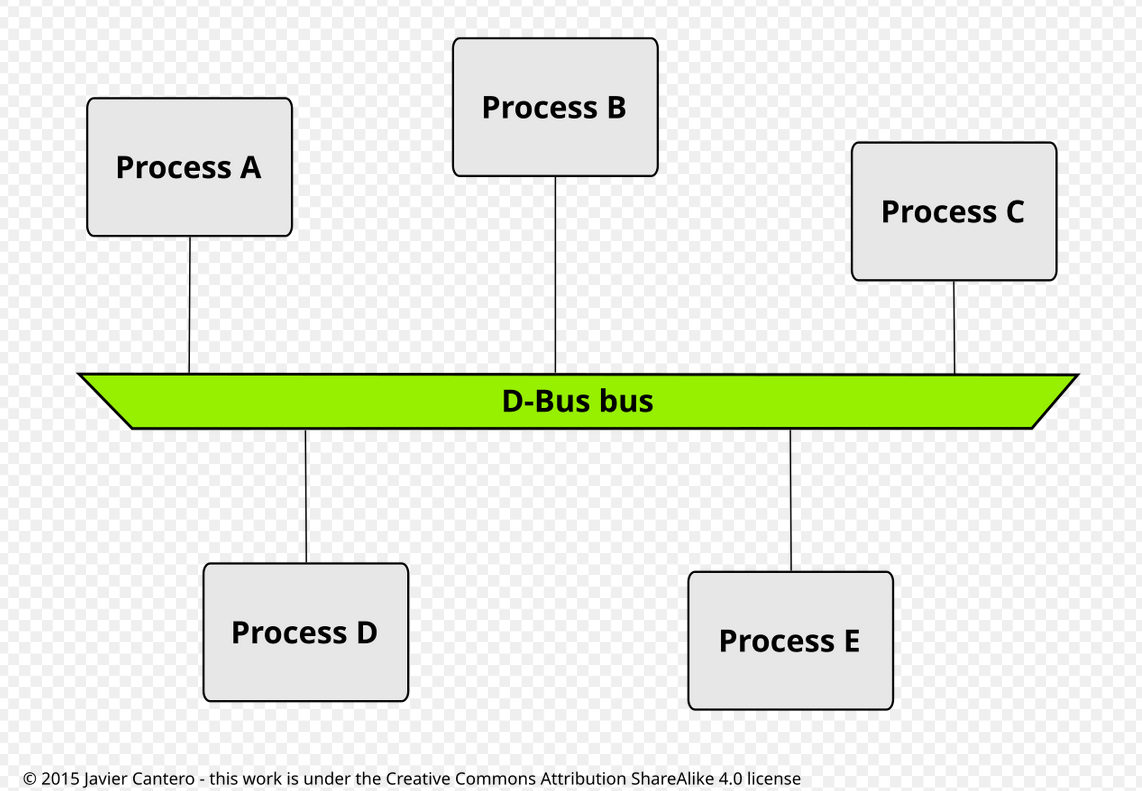
\includegraphics[width=\textwidth,height=\textheight,keepaspectratio]{dbus.png}
\end{frame}

\begin{frame}
    \frametitle{Zalety}
    \begin{itemize}
        \item Prosty
        \item Dostępność standardu w wielu językach programowania
        \item Security policy
        \item Abstrakcja połączenia
        \item Walidacja typów
    \end{itemize}
\end{frame}

\begin{frame}
    \frametitle{D-Bus bus}
    Demon do którego łączą się aplikacje. Przekierowuje
    wiadomości od aplikacji do innych aplikacji. Zaimplementowany
    w libdbus.
\end{frame}

%\begin{frame}
%    \frametitle{libdbus}
%    Niskopoziomowa biblioteka pozwalająca aplikacjom na wymianę 
%    wiadomości.
%\end{frame}

\begin{frame}
    \frametitle{System bus}
    Z poziomu użytkownika, osobna instancja dla każdego.
    \begin{itemize}
        \item GUI KDE, GNOME
        \item Aplikacje, Spotify, Firefox
        \item PulseAudio
    \end{itemize}
\end{frame}

\begin{frame}
    \frametitle{Session bus}
    Z poziomu systemu operacyjnego.
    \begin{itemize}
        \item Sieci, NetworkManager
        \item Urządzenia, UDisks, USB
        \item Uprawnienia, PolicyKit
    \end{itemize}
\end{frame}

\begin{frame}
    \frametitle{Połączenie serwisu}
    Następuje przy połączeniu do demona.
    Serwis ma przyznawaną nazwę:
    \begin{itemize}
        \item Unikalna: :1-37, :1-42
        \item Well-known name: org.Cinammon, org.mpris.MediaPlayer2.spotify
        \item Znak : zarezerwowany
    \end{itemize}
\end{frame}

\begin{frame}
    \frametitle{Obiekt}
    \begin{itemize}
        \item Wymaga określenia bus name
        \item Ścieżka do obiektu jako nazwa: 
        \begin{itemize}
            \item /org/Cinnamon 
            \item /com/Test
            \item /org/meks/Logger/1 org/meks/Logger/2
        \end{itemize}
        \item Implementuje interfejsy
        \item Implementuje sygnały i metody
    \end{itemize}
\end{frame}


\begin{frame}
    \frametitle{Interfejsy}
    Zbiór metod, sygnałów oraz właściwości (properties).
    Implementowane przez obiekty. 
    Coś jak abstract class.
\end{frame}

\begin{frame}[fragile]
    \frametitle{Proxy}
    Obiekt tworzony przez klienta jako reprezentacja
    "zdalnego" obiektu innego procesu. Niskopoziomowo tworzy
    wiadomość do serwisu z requestowanym wykonaniem metod i zwraca
    odpowiedź.

    \begin{flushleft}
        \begin{lstlisting}
Proxy proxy = new Proxy(getBusConnection(),
                         "/remote/object/path");
Object returnValue = proxy.MethodName(arg1, arg2);
        \end{lstlisting}      
    \end{flushleft}

\end{frame}

\begin{frame}
    \frametitle{Przykład}
    \begin{columns}
    \begin{column}{0.5\textwidth}
        \begin{center}
            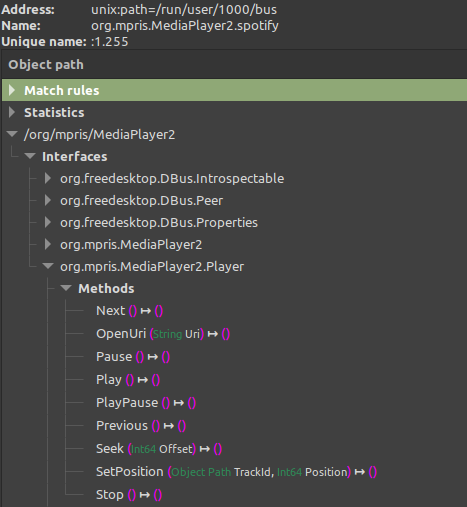
\includegraphics[width=\textwidth,height=\textheight,keepaspectratio]{service1.png}
        \end{center}
    \end{column}
    \begin{column}{0.5\textwidth}
        \begin{center}
            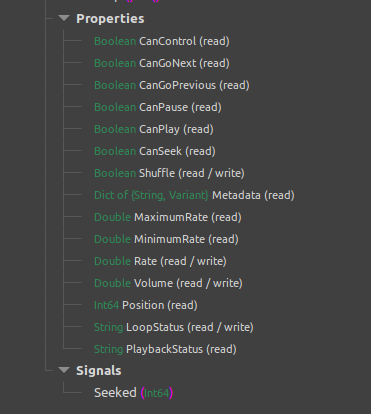
\includegraphics[width=\textwidth,height=\textheight, keepaspectratio]{example2.png}        
        \end{center}
    \end{column}
\end{columns}
\end{frame}


\begin{frame}
    \frametitle{System typów}
    \href{https://dbus.freedesktop.org/doc/dbus-specification.html}{Parę przykładów:}
    \begin{itemize}
        \item aai - tablica tablic intów
        \item a(ss) - array structów z dwoma stringami
        \item a\{sd\} - mapa klucz-string value-double
        \item v - variant, dynamiczny typ
        \item a\{sv\} - mapa z wartościami o różnych typach
    \end{itemize}
\end{frame}





% https://dbus.freedesktop.org/doc/dbus-api-design.html